%%%%%%%%%% *** The Title %%%%%%%%%%
\title[]{대기의 순환\\\small{제7장}}

\begin{frame}[plain] %title page
	\titlepage
\end{frame}



\section{대기 운동의 규모}

\begin{frame}[t]{대기 운동의 세가지 규모}
	\begin{tabular}{ll}
		\begin{minipage}[t]{0.65\textwidth}\scriptsize
			\begin{figure}[t]
				\includegraphics[trim=50 290 50 50, clip, page=218, width=\textwidth]{\bookfile}
			\end{figure}
		\end{minipage}	
		&
		\begin{minipage}[t]{0.3\textwidth} \scriptsize	
			공간 규모(수평 규모)가 커질수록 지속 시간도 길어진다.\\
			큰 소용돌이는 작은 소용돌이로 이루어져 있다
			
		\end{minipage}
	\end{tabular}
\end{frame}



\begin{frame}[t]{대기 운동의 세가지 규모}
	\begin{tabular}{ll}
		\begin{minipage}[t]{0.7\textwidth}\scriptsize
			\questionset{대규모, 중규모, 그리고 소규모 바람의 차이를 설명하고, 각각의 예를 한 가지씩 들어 설명하라.}
			\solutionset{\begin{table}[]
					\resizebox{\textwidth}{!}{%
						\begin{tabular}{c|c|c|c|c}
							\hline
							\multicolumn{2}{c|}{규모}                   & 시간 규모 & 공간 규모   & 예                \\ \hline
							\multicolumn{2}{c|}{미규모(microscale)}           & 1분    & 100m    & 난류, 회오리바람, 돌풍    \\ \hline
							\multicolumn{2}{c|}{중규모(mesoscale)}            & 1시간   & 10km    & 뇌우, 토네이도, 해륙풍    \\ \hline
							\multirow{2}{*}{대규모(macroscale)} & 종관규모(synoptic)     & 1주일   & 1000km  & 중위도 저기압, 고기압, 태풍 \\ \cline{2-5} 
							& 지구 규모(global scale) & 1달    & 10000km & 편서풍, 무역풍         \\ \hline
						\end{tabular}%
					}
			\end{table}}
		\end{minipage}	
		&
		\begin{minipage}[t]{0.25\textwidth} \scriptsize	
		
			
		\end{minipage}
	\end{tabular}
\end{frame}





\section{국지풍}



\begin{frame}[t]{회오리 바람}
	\begin{tabular}{ll}
		\begin{minipage}[t]{0.55\textwidth}\scriptsize
			\begin{figure}[t]
				\includegraphics[trim=220 450 60 90, clip, page=219, width=\textwidth]{\bookfile}
			\end{figure}
		\end{minipage}	
		&
		\begin{minipage}[t]{0.4\textwidth} \scriptsize	
			\questionset{회오리 바람(Dust devil)과 토네이도의 차이점을 설명하시오.}
			\solutionset{회오리 바람은 맑은 하늘과 높은 온도를 가진 건조한 지방에서 형성되며, 보통 토네이도보다 작고, 약하며, 짧은 주기를 가진다. \\
			뿐만 아니라 회오리 바람은 지표의 가열로 생성되지만, 토네이도는 상하간 쉬어 차이 생성된다. \\
			지표 근처 공기가 수십미터 상공 공기보다 많이 따뜻할 때 지표면 부근 기층이 불안정해진다. 이 때 지표 공기는 상승하고, 발달하는 바람 안으로 지상 부근의 공기를 끌어들인다. 회전하면서 모래, 먼지, 잔해들을 수십 미터 위 대기로 날려보내면서 회오리 바람을 육안으로 볼 수 있게 한다.}
		\end{minipage}
	\end{tabular}
\end{frame}



\begin{frame}[t]{해륙풍}
	\begin{tabular}{ll}
		\begin{minipage}[t]{0.9\textwidth}\scriptsize
			\begin{figure}[t]
				\includegraphics[trim=50 550 50 50, clip, page=220, width=\textwidth]{\bookfile}
			\end{figure}
		\end{minipage}	
		&
		\begin{minipage}[t]{0.05\textwidth} \scriptsize				
		\end{minipage}
	\end{tabular}
			
			\scriptsize
			낮 시간 동안 열대 해안은 인접한 바다보다 더 강하게 가열된다. 상층에서는 육지 위의 공기 덩이는 가열되고 팽창하므로 같은 고도에서 바다 쪽보다 높은 기압을 갖는다. \\
			이는 상공에서 공기가 바다 쪽으로 이동하게 하고, 이러한 상층 공기 이동은 해수면 근처의 압력을 높이고, 육지 위의 압력은 낮추게 된다. 그 결과로 바다에서 육지로 부는 해풍이 발생한다. \\
			유사한 과정을 반대로 적용하여 밤에 부는 육풍을 설명할 수 있다. 
\end{frame}



\begin{frame}[t]{해륙풍}
	\begin{tabular}{ll}
		\begin{minipage}[t]{0.45\textwidth}\scriptsize
			\begin{figure}[t]
				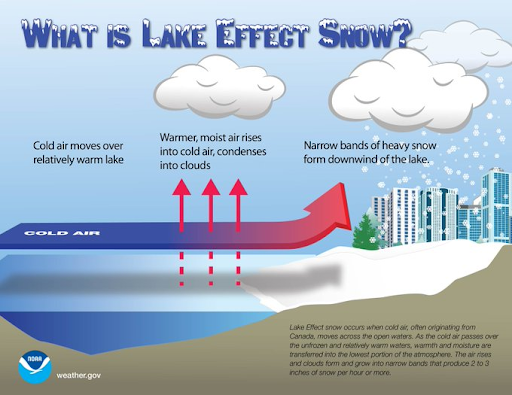
\includegraphics[width=\textwidth]{./images/lake_effect}
			\end{figure}
		\end{minipage}	
		&
		\begin{minipage}[t]{0.5\textwidth} \scriptsize	
			\questionset{가장 강한 해풍은 차가운 해류에 인접한 열대 해안을 따라 발달한다. 그 이유를 설명하라.}
			\solutionset{육지와 바다의 기온 차이가 크다면 기압 차이도 크므로 큰 기압 경도력에 의해 속력이 빠르리라 예상할 수 있다. \newline}
			
			\questionset{호수 효과가 무엇인지 설명하시오.}
			\solutionset{오대호 부근의 도시들은 여름에 호수 효과(lake effect)의 혜택을 받아, 더운 내륙보다 더 시원한 온도를 즐길 수 있다. 이는 작은 규모의 해풍이 호숫가를 따라 발달하기 때문이다. }
			
		\end{minipage}
	\end{tabular}
\end{frame}




\begin{frame}[t]{산곡풍}
	\begin{tabular}{ll}
		\begin{minipage}[t]{0.9\textwidth}\scriptsize
			\begin{figure}[t]
				\includegraphics[trim=50 30 50 580, clip, page=220, width=\textwidth]{\bookfile}
			\end{figure}
		\end{minipage}	
		&
		\begin{minipage}[t]{0.05\textwidth} \scriptsize	
			
		\end{minipage}
	\end{tabular}

			\questionset{산곡풍이 생기는 과정을 설명하시오.}
			\solutionset{낮동안 산사면은 계곡 지역보다 더 강하게 가열되어 산사면의 공기가 산사면을 따라 상승하게 되는데 이를 곡풍이라고 한다. 
				일몰 후 산사면은 계곡 지역보다 더 급격하게 공기를 냉각시키는데, 이 공기가 골짜기 쪽으로 배출되어 산풍을 만든다. }

\end{frame}




\begin{frame}[t]{산곡풍}
	\begin{tabular}{ll}
		\begin{minipage}[t]{0.55\textwidth}\scriptsize
			\begin{figure}[t]
				\includegraphics[trim=35 520 300 0, clip, page=221, width=\textwidth]{\bookfile}
			\end{figure}
		\end{minipage}	
		&
		\begin{minipage}[t]{0.4\textwidth} \scriptsize	
			\questionset{산악 지대 오후에 소나기가 내리는 원리를 설명하시오.}
			\solutionset{낮동안 산사면은 계곡 지역보다 더 강하게 가열되어 산사면의 공기가 산사면을 따라 상승하게 되는데 이 상승 기류가 강할때 구름이 발달하여 천둥 번개를 동반한 소나기가 내리기도 한다.}
			
			
		\end{minipage}
	\end{tabular}
\end{frame}




\begin{frame}[t]{여러 국지풍}
	\begin{tabular}{ll}
		\begin{minipage}[t]{0.45\textwidth}\scriptsize
			\begin{figure}[t]
				\includegraphics[trim=250 220 50 110, clip, page=223, width=0.9\textwidth]{\bookfile}
			\end{figure}
		\end{minipage}	
		&
		\begin{minipage}[t]{0.5\textwidth} \scriptsize	
			\questionset{치누크(눈 잡아먹는 바람)란 무엇인가?}
			\solutionset{보통 겨울과 봄에 콜로라도 로키 산맥의 동쪽 비탈면을 내려오며 분다. 이 바람은 건조하고 따뜻하여, 치누크가 도달한지 수 분 내에 기온이 20도 이상 상승할 수 있다. \\
			겨울의 긴 시간 동안 눈 없는 목초지를 제공하기 때문에 로키산맥 동부목장주 들에게 유익한 것으로 여겨 지기도 했으나, 봄까지 눈이 남아 있어야 땅에 수분이 공급되는데 치누크로 인해 수분이 손실되는 문제가 발생하고 있다. \\
			유사한 바람은 알프스에서의 푄, 미국 남부 캘리포니아의 산타 아나(Santa Ana)가 있다. \newline}
			
			\questionset{산타 아나(Santa Ana)란 무엇인가?}
			\solutionset{산타아나는 치누크와 같은 바람의 국지명으로 가을과 봄에 남부 캘리포니아와 북서 멕시코에 부는데 매우 뜨겁고 건조하여 산불을 촉발시킨다.}
			
		\end{minipage}
	\end{tabular}
\end{frame}




\begin{frame}[t]{여러 국지풍}
	\begin{tabular}{ll}
		\begin{minipage}[t]{0.5\textwidth}\scriptsize
			\begin{figure}[t]
				\includegraphics[trim=330 30 50 560, clip, page=221, width=\textwidth]{\bookfile}
			\end{figure}
		\end{minipage}	
		&
		\begin{minipage}[t]{0.45\textwidth} \scriptsize	
			\questionset{활강 바람(katabatic winds)이란 무엇인지 설명하시오.}
			\solutionset{높은 고도를 가진 지역에 위치한 찬 공기에서 기원한 바람으로 낮은 지역으로 이동하는 바람이다. 차갑기 때문에 밀도가 높아서 이러한 흐름을 나타낸다. \\
			초기 온도가 매우 낮으므로 단열 가열되더라도 옮겨간 지역의 공기보다 차고 무겁다.}
			
		\end{minipage}
	\end{tabular}
\end{frame}






\begin{frame}[t]{여러 국지풍}
	\begin{tabular}{ll}
		\begin{minipage}[t]{0.45\textwidth}\scriptsize
			\begin{figure}[t]
				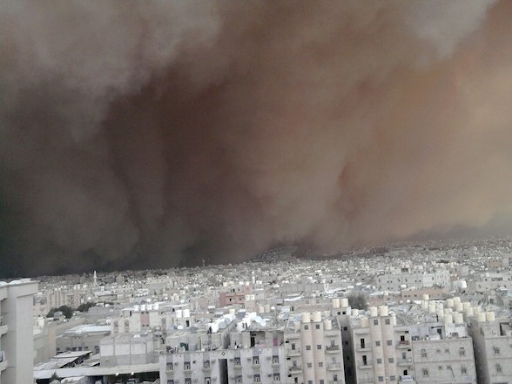
\includegraphics[width=\textwidth]{./images/haboob}
			\end{figure}
		\end{minipage}	
		&
		\begin{minipage}[t]{0.5\textwidth} \scriptsize	
			\questionset{하부브(haboob)란 무엇인가?}
			\solutionset{매년 여름 아프리카 수단의 카르툼(Khartoum)지역에 불어닥치는 거대한 모래폭풍으로 어원은 아라비아어의 ‘바람이 불다(habb)’에서 유래한 것이다.\\
				이 모래폭풍은 일종의 계절 폭풍으로 뇌우가 최종단계에 다다랐을때 생기는 하강기류에 의해 강하하는 공기가 지표면에 부딪혀 대량의 먼지를 들어올리도록 하는 것이다.
				이렇게 모인 먼지 구름은 놀라운 광경을 연출하며 시속 30마일의 속도로 이동한다.}
			
		\end{minipage}
	\end{tabular}
\end{frame}


\begin{frame}[t]{여러 국지풍}
	\begin{tabular}{ll}
		\begin{minipage}[t]{0.45\textwidth}\scriptsize
			\begin{figure}[t]
				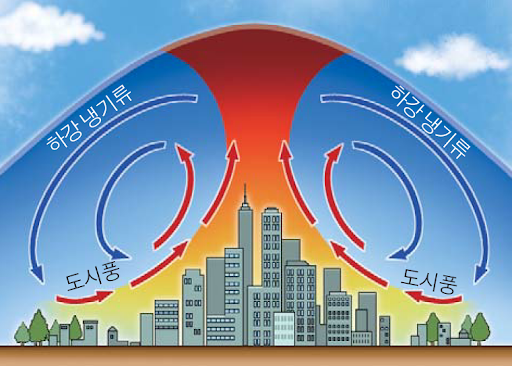
\includegraphics[width=\textwidth]{./images/ruban_wind}
			\end{figure}
		\end{minipage}	
		&
		\begin{minipage}[t]{0.5\textwidth} \scriptsize	
			\questionset{도시가 어떻게 특유의 국지풍을 생성하는 지 설명하라.}
			\solutionset{도시는 열섬 효과로 인하여 시골풍이라는 국지풍을 만들어 낸다. \\
				시골풍은 맑고 바람이 없는 밤에 상대적으로 따뜻하고 밀도가 낮은 공기가 도시 위로 이동하면서 시골에서 도시 방향으로 흐름이 생긴다.}
			
		\end{minipage}
	\end{tabular}
\end{frame}


\section{전 지구 순환}


\begin{frame}[t]{헤들리 순환}
	\begin{tabular}{ll}
		\begin{minipage}[t]{0.45\textwidth}\scriptsize
			\begin{figure}[t]
				\includegraphics[trim=50 50 330 480, clip, page=222, width=\textwidth]{\bookfile}
			\end{figure}
		\end{minipage}	
		&
		\begin{minipage}[t]{0.5\textwidth} \scriptsize	
			\questionset{George Hadley가 제안한 이상적인 전 지구 순환을 간략히 서술하라. 해들리 모델에서 고려하지 못한 점은 무엇인가?}
			\solutionset{해들리 모형에서 적도 지방의 공기는 대류권계면에 도달할 때까지 상승하다 대류권계면에서 극을 향해 이동한다. 결국 이 공기의 흐름은 극에서 냉각되어 가라앉게 되고 지표에서 적도를 향한 바람으로 변하게 된다. 차가운 공기는 적도로 이동하여 다시 가열되고 상승하게 되는 순환 과정을 거친다. \\
			하지만 이 모형은 지구의 자전을 고려하지 못했다는 단점을 가진다.}
		\end{minipage}
	\end{tabular}
\end{frame}




\begin{frame}[t]{3세포 모델}
	\begin{tabular}{ll}
		\begin{minipage}[t]{0.45\textwidth}\scriptsize
			\begin{figure}[t]
				\includegraphics[trim=350 50 0 410, clip, page=222, width=\textwidth]{\bookfile}
			\end{figure}
		\end{minipage}	
		&
		\begin{minipage}[t]{0.5\textwidth} \scriptsize	
			\questionset{위도 $20 \sim 35 \rm{^\circ} $ 사이에서 공기가 침강하는 요인 두 가지를 쓰시오.}
			\solutionset{1) 상층 공기의 복사 냉각으로 인해 밀도가 높아지는 것\\
			2) 극을 향하던 공기덩이가 점점 더 강해지는 전향력의 영향을 받아 거의 서풍으로 변하여 상층공기의 수렴을 야기함  \newline}
			
			\questionset{대기 순환의 이상적인 3세포 모델에 따르면, 우리 나라와 미국은 어떤 탁월풍 지대에 위치하는가?}
			\solutionset{우리나라와 미국 대부분은 편서풍지대(the zone of prevailing westerlies)에 위치하게 된다.}
			
		\end{minipage}
	\end{tabular}
\end{frame}




\begin{frame}[t]{대기 대순환}
	\begin{tabular}{lll}
		\begin{minipage}[t]{0.3\textwidth}\scriptsize
			\begin{figure}[t]
				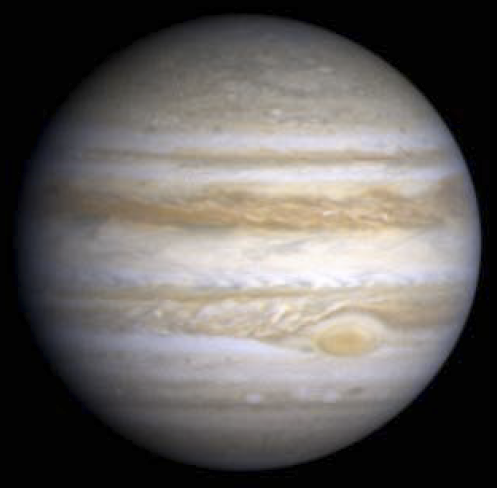
\includegraphics[width=0.98\textwidth]{./images/Jupiter1}
			\end{figure}
		\end{minipage}	
		&
		\begin{minipage}[t]{0.3\textwidth}\scriptsize
			\begin{figure}[t]
				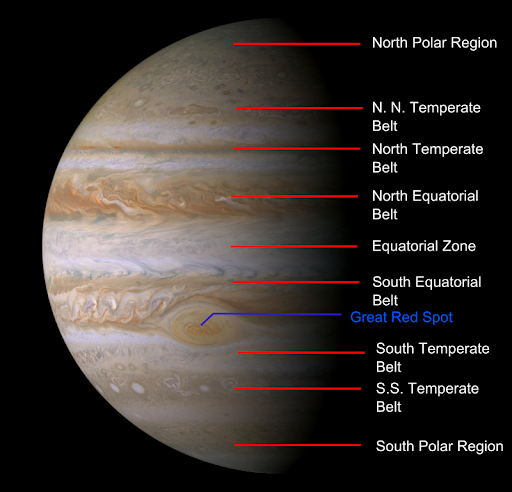
\includegraphics[width=\textwidth]{./images/Jupiter2}
			\end{figure}
		\end{minipage}	
		&
		\begin{minipage}[t]{0.3\textwidth}\scriptsize
			\begin{figure}[t]
				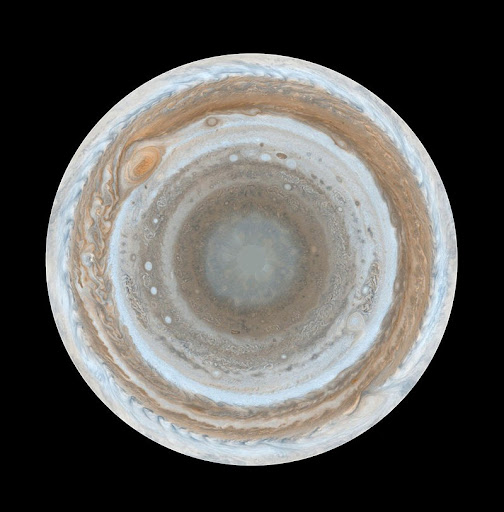
\includegraphics[width=0.95\textwidth]{./images/Jupiter3}
			\end{figure}
		\end{minipage}	

	\end{tabular}
		\newline
		
		\questionset{지구의 자전 속도가 더 빨라진다면 대기 대순환은 어떻게 변하겠는가? 특히 아열대 고압대의 위치는 어떻게 변하겠는가?}
		\solutionset{목성은 지구보다 더 빠르게 자전하기 때문에 표면에서 강한 코리올리 힘에 의해 만들어진 많은 대류 셀로 인해 생겨난 수많은 띠를 볼 수 있다. \\
			지구의 자전 속도가 빨라진다면 목성처럼 더 많은 대류 셀이 형성될 것이다. 아열대 고압대의 위치는 현재보다 저위도로 내려갈 것이다. }
		
\end{frame}





\section{바람을 구동시키는 기압대}


\begin{frame}[t]{이상화된 동서 기압대}
	\begin{tabular}{ll}
		\begin{minipage}[t]{0.65\textwidth}\scriptsize
			\begin{figure}[t]
				\includegraphics[trim=50 470 95 50, clip, page=226, width=\textwidth]{\bookfile}
			\end{figure}
		\end{minipage}	
		&
		\begin{minipage}[t]{0.3\textwidth} \scriptsize	
			\questionset{지표면이 균일한 경우와 실제 지구의 기압대를 비교하여 설명하시오.}
			\solutionset{지표면이 균일한 경우, 각 반구에 2개의 고기압대와 2개의 저기압대를 가지게 된다.(적도저기압대, 아열대고기압대, 아한대저기압대, 극고기압대) \\
			실제로는 동서 패턴이 깨짐. 주로 반영구적 고기압 및 저기압 세포들로 구성된다.}
		\end{minipage}
	\end{tabular}
\end{frame}



\begin{frame}[t]{ITCZ}
	\begin{tabular}{ll}
		\begin{minipage}[t]{0.5\textwidth}\scriptsize
			\begin{figure}[t]
				\includegraphics[trim=50 30 320 450, clip, page=226, width=\textwidth]{\bookfile}
			\end{figure}
		\end{minipage}	
		&
		\begin{minipage}[t]{0.45\textwidth} \scriptsize	
			\questionset{ITCZ이란 무엇인지 설명하시오.}
			\solutionset{(Intertropical Convergence Zone의 약자로 열대수렴대 또는 적도수렴대라고 한다.\\
				북반구의 북동무역풍과 남동무역풍의 수렴으로 인해 적도 근처에서 따뜻한 공기가 상승하는 저기압대를 말한다.}
			
		\end{minipage}
	\end{tabular}
	
\end{frame}



\begin{frame}[t]{평균 지표 기압 및 바람(1월)}
	\begin{tabular}{ll}
		\begin{minipage}[t]{0.9\textwidth}\scriptsize
			\begin{figure}[t]
				\includegraphics[trim=50 295 80 240, clip, page=227, width=\textwidth]{\bookfile}
			\end{figure}
		\end{minipage}	
		&
		\begin{minipage}[t]{0.05\textwidth} \scriptsize	
			
			
		\end{minipage}
	\end{tabular}
\end{frame}




\begin{frame}[t]{평균 지표 기압 및 바람(7월)}
	\begin{tabular}{ll}
		\begin{minipage}[t]{0.9\textwidth}\scriptsize
			\begin{figure}[t]
				\includegraphics[trim=50 40 80 500, clip, page=227, width=\textwidth]{\bookfile}
			\end{figure}
		\end{minipage}	
		&
		\begin{minipage}[t]{0.05\textwidth} \scriptsize	
			
			
		\end{minipage}
	\end{tabular}
\end{frame}




\begin{frame}[t]{평균 지표 기압 및 바람}
	\begin{tabular}{ll}
		\begin{minipage}[t]{0.55\textwidth}\scriptsize
			\begin{figure}[t]
				\includegraphics[trim=50 40 80 240, clip, page=227, width=\textwidth]{\bookfile}
			\end{figure}
		\end{minipage}	
		&
		\begin{minipage}[t]{0.4\textwidth} \scriptsize	
			\questionset{남반구 아한대 저기압 지역의 기압 패턴에 대해 설명하시오.}
			\solutionset{남반구의 바다는 대륙이 많이 위치하지 않아서, 기압 패턴을 교란할 대륙과 바다의 차등 가열의 여지가 적기 때문에 동서 방향으로 비슷한 기압 패턴을 갖는다. \newline}
			
			\questionset{1월과 7월의 북대서양에서 아열대 고기압을 비교하시오.}
			\solutionset{여름에는 뜨거운 대륙 위에 저기압이 존재한다. 기압에서 이러한 차이는 맞추기 위해 바다에서는 고기압이 생성되어야 한다. 하지만 겨울에는 대륙이 냉각되어 고기압이 존재하므로 북대서양 지역의 아열대 고기압은 1월에 더 약하다.	}
		\end{minipage}
	\end{tabular}
\end{frame}



\begin{frame}[t]{평균 지표 기압 및 바람}
	\begin{tabular}{ll}
		\begin{minipage}[t]{0.55\textwidth}\scriptsize
			\begin{figure}[t]
				\includegraphics[trim=50 40 80 240, clip, page=227, width=\textwidth]{\bookfile}
			\end{figure}
		\end{minipage}	
		&
		\begin{minipage}[t]{0.4\textwidth} \scriptsize	
			\questionset{북반구 아한대 저기압인 알류산 저기압과 아이슬란드 저기압이 겨울철에 더 자주 발생하는 이유는 무엇인가?}
			\solutionset{1월은 북반구가 겨울이므로 위도에 따른 온도 차이가 심하다. 이는 겨울철에 제트 기류의 양상에도 영향을 크게 미친다. 제트 기류는 저기압성 폭풍의 경로에 영향을 주고, 저기압성 폭풍도 겨울철에 훨씬 많이 나타난다. \newline}
			
			\questionset{북아시아 1월에 강한 고기압 세포가 발달하는 이유는 무엇인가?}
			\solutionset{겨울철 시베리아에서는 매우 혹독한 온도를 경험하게 되는데 이렇게 차가운 온도는 고기압의 주된 원인이 된다. 매우 차가운 공기의 밀도가 높기 때문에 고기압이 형성된다.}
		\end{minipage}
	\end{tabular}
\end{frame}






\section{몬순}



\begin{frame}[t]{몬순(monsoon)}
	\begin{tabular}{ll}
		\begin{minipage}[t]{0.65\textwidth}\scriptsize
			\begin{figure}[t]
				\includegraphics[trim=30 500 350 50, clip, page=229, width=0.49\textwidth]{\bookfile}
				\includegraphics[trim=30 220 350 280, clip, page=229, width=0.49\textwidth]{\bookfile}
			\end{figure}
		\end{minipage}	
		&
		\begin{minipage}[t]{0.3\textwidth} \scriptsize	
			몬순 : 계절 변화에 따라 큰 규모로 풍향이 바뀌는 것을 말한다.\\
			지표면의 불균등 가열에 의해 생성되는 기압 차이에 의해 발생한다.
			
		\end{minipage}
	\end{tabular}
\end{frame}




\begin{frame}[t]{아시아의 몬순(monsoon)}
	\begin{tabular}{ll}
		\begin{minipage}[t]{0.4\textwidth}\scriptsize
			\begin{figure}[t]
				\includegraphics[trim=30 220 350 50, clip, page=229, width=0.7\textwidth]{\bookfile}
			\end{figure}
		\end{minipage}	
		&
		\begin{minipage}[t]{0.55\textwidth} \scriptsize	
			
			\questionset{아시아 몬순은 어디에서 나타나며 어떻게 나타나는가?}
			\solutionset{아시아 몬순은 남아시아 및 남동아시아에서 일어나 인도 및 주변지역을 넘어 중국,한국, 일본에도 영향을 준다. \\
			겨울에는 러시아 북부 지역 대륙에서 차가운 공기가 축적되며 시베리아 고기압을 만들고, 이 공기가 남아시아를 가로질러 해안으로 빠져나간다. \\
			여름철에 남아시아 내륙은 강한 태양의 가열로 인해 저기압이 형성된다. 이로 인해 상승 기류가 형성되고 인도양에서 대륙으로 습한 공기가 유입되어 강수량이 크게 증가한다. 
			뿐만 아니라 ITCZ의 계절변화가 매우 큰 것도 영향 요인이 된다.}
		\end{minipage}
	\end{tabular}
\end{frame}




\begin{frame}[t]{북아메리카의 몬순}
	\begin{tabular}{ll}
		\begin{minipage}[t]{0.65\textwidth}\scriptsize
			\begin{figure}[t]
				\includegraphics[trim=305 0 50 460, clip, page=229, width=0.49\textwidth]{\bookfile}
				\includegraphics[trim=50 460 320 40, clip, page=230, width=0.49\textwidth]{\bookfile}
			\end{figure}
		\end{minipage}	
		&
		\begin{minipage}[t]{0.3\textwidth} \scriptsize	
			\questionset{북아메리카 몬순에 대해 설명하시오.}
			\solutionset{북아메리카 몬순은 건조한 봄에 이어 많은 비가 내리는 여름을 생성시키며, 주로 미국 남서부 및 멕시코 북서부에 영향을 준다. \\
			미국 남서부 지역에서 여름 기온은 매우 높아질 수 있고, 이 가열이 애리조나 주에 저기압 중심을 만든다. 이에 따라 캘리포니아만(주로)과 멕시코만(약하게)으로부터 온난 습윤 공기 유입되어 비가 많이 내린다. 실제로 멕시코 북서부 지역에서 가장 잘 나타난다. }
			
		\end{minipage}
	\end{tabular}
\end{frame}




\section{편서풍과 제트기류}




\begin{frame}[t]{편서풍 발생 원인}
	\begin{tabular}{ll}
		\begin{minipage}[t]{0.5\textwidth}\scriptsize
			\begin{figure}[t]
				\includegraphics[trim=260 50 30 490, clip, page=230, width=\textwidth]{\bookfile}
			\end{figure}
		\end{minipage}	
		&
		\begin{minipage}[t]{0.45\textwidth} \scriptsize	
			\questionset{상층에서 편서풍이 지배적인 이유는 무엇인가?}
			\solutionset{상층의 기압 경도(구배)를 보면 같은 고도에서 적도에서 극지방으로 향하는 수평 방향의 기압 경도력이 작용하게 된다. 기압 경도력에 의해 바람이 이동하게 되면 전향력이 작용하여 공기 덩이는 위도가 높아지면서 차츰 서풍으로 변하게 된다. }
						
		\end{minipage}
	\end{tabular}
\end{frame}




\begin{frame}[t]{상층 편서풍의 이상화된 기류}
	\begin{tabular}{ll}
		\begin{minipage}[t]{0.38\textwidth}\scriptsize
			\begin{figure}[t]
				\includegraphics[trim=60 420 350 50, clip, page=231, width=0.9\textwidth]{\bookfile}
			\end{figure}
		\end{minipage}	
		&
		\begin{minipage}[t]{0.57\textwidth} \scriptsize	
			\begin{figure}[t]
				\includegraphics[trim=50 480 220 50, clip, page=232, width=\textwidth]{\bookfile}
			\end{figure}
			
			
		\end{minipage}
	\end{tabular}
			\scriptsize 
			로스비 파라고 부르는 5개의 장파장 굴곡이 이 기류를 구성한다. \\
			제트기류는 이 파동 기류의 고속의 중심핵이다.
\end{frame}





\begin{frame}[t]{제트기류(Jet stream)}
	\begin{tabular}{ll}
		\begin{minipage}[t]{0.45\textwidth}\scriptsize
			\begin{figure}[t]
				\includegraphics[trim=50 190 330 310, clip, page=232, width=\textwidth]{\bookfile}
			\end{figure}
		\end{minipage}	
		&
		\begin{minipage}[t]{0.5\textwidth} \scriptsize	
			제트기류는 가파른 상층 기압 경도와 지표면에서의 큰 온도 차이로 인해 편서기류 내에서 발생하는 강하고 빠른 바람이다.\\
			매우 좁은 지역에 걸쳐 큰 온도 차이를 갖는 지역에서 빠른 상층 바람이 발생한다. \\
			한대 제트기류(Polar jet stream) : 가장 일반적인 제트기류로 한대 전선대에 위치\\
			
		\end{minipage}
	\end{tabular}
\end{frame}


\begin{frame}[t]{제트기류(Jet stream)}
	\begin{tabular}{ll}
		\begin{minipage}[t]{0.5\textwidth}\scriptsize
			\begin{figure}[t]
				\includegraphics[trim=345 10 20 510, clip, page=232, width=\textwidth]{\bookfile}
			\end{figure}
		\end{minipage}	
		&
		\begin{minipage}[t]{0.45\textwidth} \scriptsize	
			\questionset{상층 일기도에서 기압 분포를 나타내는 방법을 설명하라. 제트기류는 어떤 상층 일기도에 나타나는가?}
			\solutionset{상층에서는 특정 고도에서 기압을 나타내는 대신, 특정 기압을 갖는 등고선으로 기압 분포를 나타낸다. \\
			특정 기압을 갖는 고도가 높은 곳은 사실 고기압에 해당되며, 고도가 낮은 곳은 저기압에 해당된다.\\
			제트기류는 대류권계면 부근이므로  $300 \rm{~hPa}$(여름철에는 $200 \rm{~hPa}$) 상층 일기도를 분석한다. }		
			
		\end{minipage}
	\end{tabular}
\end{frame}



\begin{frame}[t]{한대 제트기류(polar jet stream)}
	\begin{tabular}{ll}
		\begin{minipage}[t]{0.4\textwidth}\scriptsize
			\begin{figure}[t]
				\includegraphics[trim=10 460 350 50, clip, page=233, width=\textwidth]{\bookfile}
			\end{figure}
		\end{minipage}	
		&
		\begin{minipage}[t]{0.55\textwidth} \scriptsize	
				\questionset{한대 제트기류가 빠를 것으로 예상되는 계절은 언제인가?}
				\solutionset{지표에서 온도 차이가 크면 상층에서의 기압경도력도 커지고 편서풍의 세기도 빨라진다. 중위도 지방에서는 겨울철에 기온 차이가 커서 가장 빠른 편서풍이 나타난다.
				제트기류는 여름에는 북쪽으로 이동하고, 겨울에는 남쪽으로 이동한다. \newline }
				
				\questionset{한대 제트기류가 중위도 날씨에 미치는 영향을 설명하시오.}
				\solutionset{1) 지상 폭풍들의 회전 운동에 필요한 에너지 공급 및 폭풍 이동 경로에 영향\\
				2) 뇌우와 토네이도의 발생 위치 변화 : 멕시코만 접한 주에서는 대부분의 뇌우와 토네이도가 2월에 발생하지만, 여름철에는 북부 대평원과 5대호 지역으로 변화\\
				3) 지표의 기온과 습도에 영향 : 원래 위치보다 더 적도 쪽에 위치하면 날씨가 더 춥고 건조하며, 더 극 쪽으로 이동하면 정상보다 더 따뜻하고 습하게 됨.}
				
		\end{minipage}
	\end{tabular}
\end{frame}




\begin{frame}[t]{아열대 제트기류(subtropical jet stream)}
	\begin{tabular}{ll}
		\begin{minipage}[t]{0.45\textwidth}\scriptsize
			\begin{figure}[t]
				\includegraphics[trim=320 525 50 50, clip, page=233, width=\textwidth]{\bookfile}
			\end{figure}
		\end{minipage}	
		&
		\begin{minipage}[t]{0.5\textwidth} \scriptsize	
			아열대 제트기류(subtropical jet stream) : 주로 겨울철에 나타나고 한대 제트보다는 더 느리게 서에서 동으로 분다.\\
			위도 $25 \rm{^\circ}$, 고도 약 $13 \rm{~km}$에 중심을 두고 있다. \\
			북반구 겨울에 아열대 제트가 북쪽을 지나가면, 멕시코 연안이나 플로리다 남부 지역에 온난 다습한 조건을 주게 된다.\\
			
		\end{minipage}
	\end{tabular}
\end{frame}




\begin{frame}[t]{편서풍 파동의 주기적인 변화}
	\begin{tabular}{ll}
		\begin{minipage}[t]{0.5\textwidth}\scriptsize
			\begin{figure}[t]
				\includegraphics[trim=30 30 270 390, clip, page=233, width=\textwidth]{\bookfile}
			\end{figure}
		\end{minipage}	
		&
		\begin{minipage}[t]{0.45\textwidth} \scriptsize	
			\questionset{편서풍 파동의 역할은 무엇인가?}
			\solutionset{편서풍 파동은 따뜻한 공기는 극으로 이동하도록 하고 차가운 공기는 적도 쪽으로 이동하도록 한다. 결국 에너지 재분배를 통해 온도 구배가 작아지고 상층의 파동도 줄게 된다.}
			
		\end{minipage}
	\end{tabular}
\end{frame}




\begin{frame}[t]{회전 원통 실험}
	\begin{tabular}{ll}
		\begin{minipage}[t]{0.4\textwidth}\scriptsize
			\begin{figure}[t]
				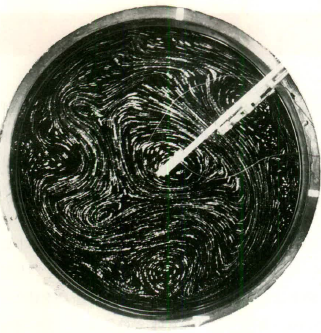
\includegraphics[width=\textwidth]{./images/rotate_cylinder}
			\end{figure}
		\end{minipage}	
		&
		\begin{minipage}[t]{0.55\textwidth} \scriptsize	
			\questionset{회전 원통 실험이란 무엇이며, 우리는 이 실험으로부터 무엇을 알 수 있는가?}
			\solutionset{자전하는 지구에서 적도지방과 극지방의 온도차에 의해 생성되는 기압경도력에 의해 형성된 편서풍이 기압과 온도차의 변화에 따라 파동의 모양이 달라지는 것을 모사하기 위한 실험 장치이다. \\
			따뜻한 적도 지방을 모사하기 위해 회전 원통의 바깥쪽은 가열하고, 극 지방을 모사하기 위해 중심부는 냉각시킨 상태에서 회전수를 조절하면서 생기는 파동의 모양을 관찰하는데 흐름을 좀 더 가시적으로 확인하기 위해 색소나 부유하는 물체, 색깔있는 입자 등을 넣어준다. \\
			회전 원통 실험에서 회전 속도의 변화와 온도차에 따라 편서풍 파동의 모양이 달라짐을 확인할 수 있었고 이를 통해 계절별로 나타나는 편서풍 파동의 파수 변화를 설명할 수 있었다.}
		
		\end{minipage}
	\end{tabular}
\end{frame}



\section{전 지구 바람과 해류}


\begin{frame}[t]{바람과 해류}
	\begin{tabular}{ll}
		\begin{minipage}[t]{0.9\textwidth}\scriptsize
			\begin{figure}[t]
				\includegraphics[trim=30 410 50 50, clip, page=235, width=0.8\textwidth]{\bookfile}
			\end{figure}
		\end{minipage}	
		&
		\begin{minipage}[t]{0.05\textwidth} \scriptsize	
						
		\end{minipage}
	\end{tabular}

			\questionset{환류가 무엇이며, 어떤 종류가 있는지 쓰시오.}
			\solutionset{지구상의 표층 해류들은 환류라고 부르는 원형의 해류 시스템을 이루고 있으며, 남대서양 및 북대서양, 남태평양 및 북태평양, 인도양에 위치하고 있다. 환류는 거의 원형이며 아열대 고기압 시스템들에 중심을 두고 있다.}

\end{frame}


\begin{frame}[t]{바람과 해류}
	\begin{tabular}{ll}
		\begin{minipage}[t]{0.55\textwidth}\scriptsize
			\begin{figure}[t]
				\includegraphics[trim=30 410 50 50, clip, page=235, width=\textwidth]{\bookfile}
			\end{figure}
		\end{minipage}	
		&
		\begin{minipage}[t]{0.4\textwidth} \scriptsize	
			\questionset{난류가 기후에 미치는 영향을 설명하시오.}
			\solutionset{난류의 하나인 북대서양 해류는 영국과 서유럽의 지역의 겨울철 기온을 동 위도 다른 지역보다 따뜻하게 유지 시켜 준다.\\
			즉, 난류가 흐르는 지역은 동위도 다른 지역보다 겨울철 기온을 높여주는 역할을 한다. (멕시코 만류, 쿠로시오 해류 등)}
		\end{minipage}
	\end{tabular}	
\end{frame}





\begin{frame}[t]{바람과 해류}
	\begin{tabular}{ll}
		\begin{minipage}[t]{0.5\textwidth}\scriptsize
			\begin{figure}[t]
				\includegraphics[trim=320 30 50 520, clip, page=235, width=\textwidth]{\bookfile}
			\end{figure}
		\end{minipage}	
		&
		\begin{minipage}[t]{0.45\textwidth} \scriptsize	
			\questionset{한류가 기후에 미치는 영향을 설명하시오.}
			\solutionset{한류는 열대 지역과 여름철 중위도 지역에 영향을 크게 미친다. \\
			예를들어 남아프리카 서해안을 흐르는 벵겔라 해류는 열대의 열을 식혀 준다. 즉, 동위도의 다른 지역에 비해 한류가 흐르는 지역의 여름 기온을 낮춰준다.
			대륙의 서해안을 따라 사막이 존재하는 곳에서는 한류에 의해 하층 대기가 냉각되기 때문에 공기는 더 안정해지고 상승 운동이 억제되어 구름 형성을 방해한다.이로 인해 건조도는 더 심화된다. \\
			반면 기온을 이슬점 온도에 근접시키게 되어 상대습도를 높이고 안개를 발생시켜 일부 아열대 사막들을 비교적 선선하고 습한 곳으로 변질시킨다.}
		\end{minipage}
	\end{tabular}
\end{frame}




\begin{frame}[t]{바람과 용승}
	\begin{tabular}{ll}
		\begin{minipage}[t]{0.9\textwidth}\scriptsize
			\begin{figure}[t]
				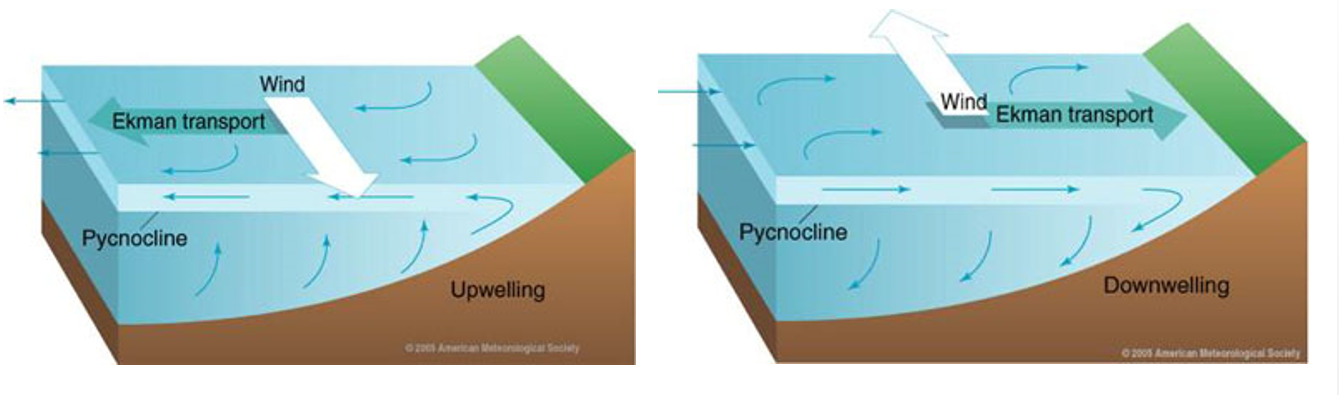
\includegraphics[width=\textwidth]{./images/upwelling}
			\end{figure}
		\end{minipage}	
		&
		\begin{minipage}[t]{0.05\textwidth}					
		\end{minipage}
	\end{tabular}
		
		\questionset{용승이란 무엇이며 해양 생물에 어떤 역할을 하는가?}
		\solutionset{용승이란 좀 더 깊은 층에 있던 차가운 물이 상승하여 해수 표면에 있는 따뜻한 물을 대신하는 현상을 말한다. 표면에 있던 물이 해변으로부터 멀리 이동하면서 질산염이나 인산염과 같은 영양 염류가 풍부한 심층의 물로 대체되면서 플랑크톤이 풍부해지고 이로 인해 해양생물이 풍족해진다.}

\end{frame}




\section{엘니뇨, 라니냐, 남방진동}




\begin{frame}[t]{엘니뇨와 라니냐}
	\begin{tabular}{ll}
		\begin{minipage}[t]{0.55\textwidth}\scriptsize
			\begin{figure}[t]
				\includegraphics[trim=50 410 250 50, clip, page=237, width=\textwidth]{\bookfile}
			\end{figure}
		\end{minipage}	
		&
		\begin{minipage}[t]{0.4\textwidth} \scriptsize	
			엘니뇨: 무역풍의 약화로 동태평양의 용승이 약화되어  동태평양의 해수 온도가 상승하는 현상\\
			라니냐: 무역풍의 강화로 동태평양의 용승이 강화되어 동태평양의 해수 온도가 더욱 하강하는 현상
			
		\end{minipage}
	\end{tabular}
\end{frame}




\begin{frame}[t]{라니냐와 수온 편차}
	\begin{tabular}{ll}
		\begin{minipage}[t]{0.45\textwidth}\scriptsize
			\begin{figure}[t]
				\includegraphics[trim=330 20 50 440, clip, page=237, width=\textwidth]{\bookfile}
			\end{figure}
		\end{minipage}	
		&
		\begin{minipage}[t]{0.45\textwidth}
			\begin{figure}[t]
				\includegraphics[trim=0 480 250 50, clip, page=239, width=0.9\textwidth]{\bookfile}
			\end{figure}
		
			\questionset{그림은 2011년 1월에 일어난 오스트레일리아 퀸즈랜드의 홍수 모습이다. 엘리뇨와 라니냐 중 어떤 현상이 나타났을 때인가? }
			\solutionset{라니냐 시기에 호주는 해수면 온도가 높아지고 호우가 발생한다. 
			오른쪽 그림을 보면 라니냐로 동태평양의 수온은 낮고, 호주의 수온은 높아진 것을 확인할 수 있다.}
		
		\end{minipage}
	\end{tabular}
\end{frame}





\begin{frame}[t]{엘니뇨}
	\begin{tabular}{ll}
		\begin{minipage}[t]{0.6\textwidth}\scriptsize
			\begin{figure}[t]
				\includegraphics[trim=250 420 30 50, clip, page=238, width=\textwidth]{\bookfile}
			\end{figure}
		\end{minipage}	
		&
		\begin{minipage}[t]{0.35\textwidth} \scriptsize	
			\questionset{열대 태평양에서의 대형 엘니뇨 사건이 지구의 다른 지역들의 날씨에 어떻게 영향을 미치는지 기술하라.}
			\solutionset{엘니뇨가 일어나면 일반적으로 페루와 에콰도르와 같이 건조한 지역은 습윤해지는 반면 인도네시아, 오스트레일리아, 필리핀과 같은 지역은 가뭄을 유발한다.\\ 
			미국 북부 지역과 캐나다 지역은 평년보다 따뜻한 겨울이 나타나고, 대서양의 허리케인의 발생 빈도가 감소하는 효과도 있었으며, 맹렬한 겨울폭풍이 캘리포니아 해안을 강타하기도 했다.}
			
		\end{minipage}
	\end{tabular}
\end{frame}



\begin{frame}[t]{라니냐}
	\begin{tabular}{ll}
		\begin{minipage}[t]{0.6\textwidth}\scriptsize
			\begin{figure}[t]
				\includegraphics[trim=250 70 30 380, clip, page=238, width=\textwidth]{\bookfile}
			\end{figure}
		\end{minipage}	
		&
		\begin{minipage}[t]{0.35\textwidth} \scriptsize	
			\questionset{라니냐는 엘니뇨와 어떻게 다른가?}
			\solutionset{라니냐는 엘니뇨가 일어나지 않는 정상 상태를 더욱 강화한다. 예를 들어 페루 해류가 강해지고 용승이 증가하고, 서태평양의 해수의 온도는 증가하게 된다. \newline}
			
			\questionset{라니냐가 발생하면 지구 다른 지역의 날씨에 어떤 영향을 미치는가?}
			\solutionset{오스트레일리아 북부와 인도네시아에는 홍수를 초래시키게 되며, 남아메리카 서해안 지역은 건조한 상태를 만든다. 반면, 남아메리카 서해안의 용승이 강화되어 어획량 증가에 기여한다. 한편, 미국 북서부를 더 차고 습하게 만들며, 남서부 및 남동부에서는 비정상적으로 따뜻한 날씨를 만들기도 한다. }
		\end{minipage}
	\end{tabular}
\end{frame}




\begin{frame}[t]{남방 진동(Southern Oscillation)}
	\begin{tabular}{ll}
		\begin{minipage}[t]{0.65\textwidth}\scriptsize
			\begin{figure}[t]
				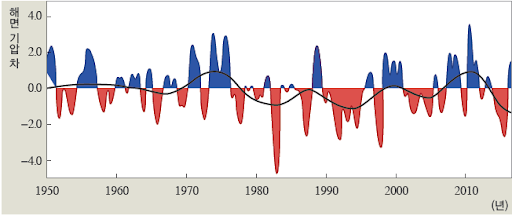
\includegraphics[width=\textwidth]{./images/SO}
			\end{figure}
		\end{minipage}	
		&
		\begin{minipage}[t]{0.3\textwidth} \scriptsize	
			\questionset{남방 진동이 무엇인지 설명하시오.}
			\solutionset{엘니뇨와 라니냐 현상이 전 지구적인 기압 패턴 변화와 밀접히 연관되어 있는데, 동태평양과 서태평양 간의 기압 시소 패턴을 남방진동(Southern Oscillation)이라 부른다. \\
			그 주기는 약 $3 \sim 7$년 이다.}
		\end{minipage}
	\end{tabular}
\end{frame}







\section{전 지구 강수 분포}

\begin{frame}[t]{강수 분포}
	\begin{tabular}{ll}
		\begin{minipage}[t]{0.28\textwidth}\scriptsize
			\begin{figure}[t]
				\includegraphics[trim=50 365 350 50, clip, page=241, width=\textwidth]{\bookfile}
			\end{figure}
		\end{minipage}	
		&
		\begin{minipage}[t]{0.62\textwidth} \scriptsize	
			\begin{figure}[t]
				\includegraphics[trim=50 20 10 400, clip, page=240, width=\textwidth]{\bookfile}
			\end{figure}
			
		\end{minipage}
	\end{tabular}

		\questionset{전지구 규모의 바람과 기압 시스템 이외에 세계 강수 분포에 영향을 미치는 요소에는 무엇이 추가로 있는가?}
		\solutionset{기온, 산맥, 대륙도, 해류}

\end{frame}




\begin{frame}[t]{아열대 고기압}
	\begin{tabular}{ll}
		\begin{minipage}[t]{0.5\textwidth}\scriptsize
			\begin{figure}[t]
				\includegraphics[trim=50 480 340 50, clip, page=242, width=\textwidth]{\bookfile}
			\end{figure}
		\end{minipage}	
		&
		\begin{minipage}[t]{0.45\textwidth} \scriptsize	
			\questionset{아열대 고기압에서 동서 강수 패턴이 차이를 나타내는 이유를 설명하시오.}
			\solutionset{아열대 고기압의 동쪽과 서쪽의 상이한 특성에 기인한 것이다. 동쪽에서는 하강운동이 현저하여 안정한 대기 상태를 만들고, 보통 겨울에 대양의 동쪽에 몰리는 경향이 있어서 아열대 고기압에 접해 있는 대륙들의 서쪽 지역이 건조하게 된다. \\
			반면 고기압들의 서쪽 지역에서는 하강운동이 덜 현저하여 온수역을 횡단하는 공기가 증발을 통해 수분을 얻게 되어 불안정도가 증가한다. 즉, 아열대 고기압 서쪽에 위치한 대륙에는 연중 충분한 강수가 내린다. }
		\end{minipage}
	\end{tabular}
\end{frame}




